\batchmode


\documentclass{article}
\RequirePackage{ifthen}



\usepackage{html}
\usepackage{nummargins}

%
\providecommand{\labnumber}{1}\input{lab1-defs}
\input{lab-defs}

\usepackage{makeidx}
\usepackage{graphicx}   
\usepackage{color}  

\usepackage{changebar}
\usepackage{natbib}

\usepackage{rcs,fancyheadings}
\pagestyle{fancy} 
\RCS $RCSfile: images.tex,v $\RCS $Revision: 1.1.1.1 $\RCS $Date: 2002/01/02 19:36:28 $\lhead{\RCSRCSfile} 
\rhead{Lab 1: page~\thepage } 
\chead{\RCSRevision}
\lfoot{}
\cfoot{}
\rfoot{}

\title{Laboratory \#1:\\
  An Introduction to the Numerical Solution of
  Differential Equations: Discretization
}
\author{John M. Stockie}\date{Date printed: \today \\
{\footnotesize [RCS version: \RCSRevision\ $-$\ \RCSDate]}
} 

\makeindex
\makeglossary



\pagecolor[gray]{.7}

\usepackage[]{inputenc}



\makeatletter
\AtBeginDocument{\makeatletter
\input /nfs/roc/home/phil/www/numeric/labs/lab1/lab1/lab1.aux
\makeatother
}

\makeatletter
\count@=\the\catcode`\_ \catcode`\_=8 
\newenvironment{tex2html_wrap}{}{}%
\catcode`\<=12\catcode`\_=\count@
\newcommand{\providedcommand}[1]{\expandafter\providecommand\csname #1\endcsname}%
\newcommand{\renewedcommand}[1]{\expandafter\providecommand\csname #1\endcsname{}%
  \expandafter\renewcommand\csname #1\endcsname}%
\newcommand{\newedenvironment}[1]{\newenvironment{#1}{}{}\renewenvironment{#1}}%
\let\newedcommand\renewedcommand
\let\renewedenvironment\newedenvironment
\makeatother
\let\mathon=$
\let\mathoff=$
\ifx\AtBeginDocument\undefined \newcommand{\AtBeginDocument}[1]{}\fi
\newbox\sizebox
\setlength{\hoffset}{0pt}\setlength{\voffset}{0pt}
\addtolength{\textheight}{\footskip}\setlength{\footskip}{0pt}
\addtolength{\textheight}{\topmargin}\setlength{\topmargin}{0pt}
\addtolength{\textheight}{\headheight}\setlength{\headheight}{0pt}
\addtolength{\textheight}{\headsep}\setlength{\headsep}{0pt}
\setlength{\textwidth}{349pt}
\newwrite\lthtmlwrite
\makeatletter
\let\realnormalsize=\normalsize
\global\topskip=2sp
\def\preveqno{}\let\real@float=\@float \let\realend@float=\end@float
\def\@float{\let\@savefreelist\@freelist\real@float}
\def\liih@math{\ifmmode$\else\bad@math\fi}
\def\end@float{\realend@float\global\let\@freelist\@savefreelist}
\let\real@dbflt=\@dbflt \let\end@dblfloat=\end@float
\let\@largefloatcheck=\relax
\let\if@boxedmulticols=\iftrue
\def\@dbflt{\let\@savefreelist\@freelist\real@dbflt}
\def\adjustnormalsize{\def\normalsize{\mathsurround=0pt \realnormalsize
 \parindent=0pt\abovedisplayskip=0pt\belowdisplayskip=0pt}%
 \def\phantompar{\csname par\endcsname}\normalsize}%
\def\lthtmltypeout#1{{\let\protect\string \immediate\write\lthtmlwrite{#1}}}%
\newcommand\lthtmlhboxmathA{\adjustnormalsize\setbox\sizebox=\hbox\bgroup\kern.05em }%
\newcommand\lthtmlhboxmathB{\adjustnormalsize\setbox\sizebox=\hbox to\hsize\bgroup\hfill }%
\newcommand\lthtmlvboxmathA{\adjustnormalsize\setbox\sizebox=\vbox\bgroup %
 \let\ifinner=\iffalse \let\)\liih@math }%
\newcommand\lthtmlboxmathZ{\@next\next\@currlist{}{\def\next{\voidb@x}}%
 \expandafter\box\next\egroup}%
\newcommand\lthtmlmathtype[1]{\gdef\lthtmlmathenv{#1}}%
\newcommand\lthtmllogmath{\lthtmltypeout{l2hSize %
:\lthtmlmathenv:\the\ht\sizebox::\the\dp\sizebox::\the\wd\sizebox.\preveqno}}%
\newcommand\lthtmlfigureA[1]{\let\@savefreelist\@freelist
       \lthtmlmathtype{#1}\lthtmlvboxmathA}%
\newcommand\lthtmlpictureA{\bgroup\catcode`\_=8 \lthtmlpictureB}%
\newcommand\lthtmlpictureB[1]{\lthtmlmathtype{#1}\egroup
       \let\@savefreelist\@freelist \lthtmlhboxmathB}%
\newcommand\lthtmlpictureZ[1]{\hfill\lthtmlfigureZ}%
\newcommand\lthtmlfigureZ{\lthtmlboxmathZ\lthtmllogmath\copy\sizebox
       \global\let\@freelist\@savefreelist}%
\newcommand\lthtmldisplayA{\bgroup\catcode`\_=8 \lthtmldisplayAi}%
\newcommand\lthtmldisplayAi[1]{\lthtmlmathtype{#1}\egroup\lthtmlvboxmathA}%
\newcommand\lthtmldisplayB[1]{\edef\preveqno{(\theequation)}%
  \lthtmldisplayA{#1}\let\@eqnnum\relax}%
\newcommand\lthtmldisplayZ{\lthtmlboxmathZ\lthtmllogmath\lthtmlsetmath}%
\newcommand\lthtmlinlinemathA{\bgroup\catcode`\_=8 \lthtmlinlinemathB}
\newcommand\lthtmlinlinemathB[1]{\lthtmlmathtype{#1}\egroup\lthtmlhboxmathA
  \vrule height1.5ex width0pt }%
\newcommand\lthtmlinlineA{\bgroup\catcode`\_=8 \lthtmlinlineB}%
\newcommand\lthtmlinlineB[1]{\lthtmlmathtype{#1}\egroup\lthtmlhboxmathA}%
\newcommand\lthtmlinlineZ{\egroup\expandafter\ifdim\dp\sizebox>0pt %
  \expandafter\centerinlinemath\fi\lthtmllogmath\lthtmlsetinline}
\newcommand\lthtmlinlinemathZ{\egroup\expandafter\ifdim\dp\sizebox>0pt %
  \expandafter\centerinlinemath\fi\lthtmllogmath\lthtmlsetmath}
\newcommand\lthtmlindisplaymathZ{\egroup %
  \centerinlinemath\lthtmllogmath\lthtmlsetmath}
\def\lthtmlsetinline{\hbox{\vrule width.1em \vtop{\vbox{%
  \kern.1em\copy\sizebox}\ifdim\dp\sizebox>0pt\kern.1em\else\kern.3pt\fi
  \ifdim\hsize>\wd\sizebox \hrule depth1pt\fi}}}
\def\lthtmlsetmath{\hbox{\vrule width.1em\kern-.05em\vtop{\vbox{%
  \kern.1em\kern0.8 pt\hbox{\hglue.17em\copy\sizebox\hglue0.8 pt}}\kern.3pt%
  \ifdim\dp\sizebox>0pt\kern.1em\fi \kern0.8 pt%
  \ifdim\hsize>\wd\sizebox \hrule depth1pt\fi}}}
\def\centerinlinemath{%
  \dimen1=\ifdim\ht\sizebox<\dp\sizebox \dp\sizebox\else\ht\sizebox\fi
  \advance\dimen1by.5pt \vrule width0pt height\dimen1 depth\dimen1 
 \dp\sizebox=\dimen1\ht\sizebox=\dimen1\relax}

\def\lthtmlcheckvsize{\ifdim\ht\sizebox<\vsize 
  \ifdim\wd\sizebox<\hsize\expandafter\hfill\fi \expandafter\vfill
  \else\expandafter\vss\fi}%
\providecommand{\selectlanguage}[1]{}%
\makeatletter \tracingstats = 1 


\begin{document}
\pagestyle{empty}\thispagestyle{empty}\lthtmltypeout{}%
\lthtmltypeout{latex2htmlLength hsize=\the\hsize}\lthtmltypeout{}%
\lthtmltypeout{latex2htmlLength vsize=\the\vsize}\lthtmltypeout{}%
\lthtmltypeout{latex2htmlLength hoffset=\the\hoffset}\lthtmltypeout{}%
\lthtmltypeout{latex2htmlLength voffset=\the\voffset}\lthtmltypeout{}%
\lthtmltypeout{latex2htmlLength topmargin=\the\topmargin}\lthtmltypeout{}%
\lthtmltypeout{latex2htmlLength topskip=\the\topskip}\lthtmltypeout{}%
\lthtmltypeout{latex2htmlLength headheight=\the\headheight}\lthtmltypeout{}%
\lthtmltypeout{latex2htmlLength headsep=\the\headsep}\lthtmltypeout{}%
\lthtmltypeout{latex2htmlLength parskip=\the\parskip}\lthtmltypeout{}%
\lthtmltypeout{latex2htmlLength oddsidemargin=\the\oddsidemargin}\lthtmltypeout{}%
\makeatletter
\if@twoside\lthtmltypeout{latex2htmlLength evensidemargin=\the\evensidemargin}%
\else\lthtmltypeout{latex2htmlLength evensidemargin=\the\oddsidemargin}\fi%
\lthtmltypeout{}%
\makeatother
\setcounter{page}{1}
\onecolumn

% !!! IMAGES START HERE !!!

{\newpage\clearpage
\lthtmlinlinemathA{tex2html_wrap_inline1883}%
$T(t)$%
\lthtmlinlinemathZ
\lthtmlcheckvsize\clearpage}

{\newpage\clearpage
\lthtmlinlinemathA{tex2html_wrap_inline1885}%
$T_0=-10,15,20,30$%
\lthtmlinlinemathZ
\lthtmlcheckvsize\clearpage}

{\newpage\clearpage
\lthtmlinlinemathA{tex2html_wrap_inline1887}%
$\lambda =10^{-5}$%
\lthtmlinlinemathZ
\lthtmlcheckvsize\clearpage}

{\newpage\clearpage
\lthtmlinlinemathA{tex2html_wrap_inline1889}%
$T_a=20$%
\lthtmlinlinemathZ
\lthtmlcheckvsize\clearpage}

{\newpage\clearpage
\lthtmlinlinemathA{tex2html_wrap_inline1895}%
$\lambda $%
\lthtmlinlinemathZ
\lthtmlcheckvsize\clearpage}

{\newpage\clearpage
\lthtmlinlinemathA{tex2html_wrap_inline1897}%
$\lambda (T)$%
\lthtmlinlinemathZ
\lthtmlcheckvsize\clearpage}

{\newpage\clearpage
\lthtmlinlinemathA{tex2html_wrap_inline1901}%
$\alpha =0.2$%
\lthtmlinlinemathZ
\lthtmlcheckvsize\clearpage}

{\newpage\clearpage
\lthtmlinlinemathA{tex2html_wrap_inline1904}%
$f$%
\lthtmlinlinemathZ
\lthtmlcheckvsize\clearpage}

{\newpage\clearpage
\lthtmlinlinemathA{tex2html_wrap_inline1906}%
$g$%
\lthtmlinlinemathZ
\lthtmlcheckvsize\clearpage}

{\newpage\clearpage
\lthtmlinlinemathA{tex2html_wrap_inline1912}%
$t_i=t_0+i\unhbox \voidb@x \hbox {$\Delta t$}{}$%
\lthtmlinlinemathZ
\lthtmlcheckvsize\clearpage}

{\newpage\clearpage
\lthtmlinlinemathA{tex2html_wrap_inline1914}%
$i=0,1,2,\dots  $%
\lthtmlinlinemathZ
\lthtmlcheckvsize\clearpage}

{\newpage\clearpage
\lthtmlinlinemathA{tex2html_wrap_inline1918}%
$y=x^3-5x$%
\lthtmlinlinemathZ
\lthtmlcheckvsize\clearpage}

{\newpage\clearpage
\lthtmlinlinemathA{tex2html_wrap_inline1920}%
$\Delta t$%
\lthtmlinlinemathZ
\lthtmlcheckvsize\clearpage}

{\newpage\clearpage
\lthtmlinlinemathA{tex2html_wrap_inline1926}%
$(x_i,t_n)$%
\lthtmlinlinemathZ
\lthtmlcheckvsize\clearpage}

{\newpage\clearpage
\lthtmlinlinemathA{tex2html_wrap_inline50}%
$RCSfile: images.tex,v $%
\lthtmlinlinemathZ
\lthtmlcheckvsize\clearpage}

{\newpage\clearpage
\lthtmlinlinemathA{tex2html_wrap_inline52}%
$Revision: 1.1.1.1 $%
\lthtmlinlinemathZ
\lthtmlcheckvsize\clearpage}

{\newpage\clearpage
\lthtmlinlinemathA{tex2html_wrap_inline54}%
$Date: 2002/01/02 19:36:28 $%
\lthtmlinlinemathZ
\lthtmlcheckvsize\clearpage}

{\newpage\clearpage
\lthtmlinlinemathA{tex2html_wrap_inline56}%
$-$%
\lthtmlinlinemathZ
\lthtmlcheckvsize\clearpage}


%
\providecommand{\ie}{i.e.~}%


%
\providecommand{\eg}{e.g.~}%


%
\providecommand{\dt}{\mbox{$\Delta t$}{}}%


%
\providecommand{\yi}{\mbox{$y_i$}{}}%


%
\providecommand{\ti}{\mbox{$t_i$}{}}%


%
\providecommand{\eqref}[1]{(\ref{#1})}%

\stepcounter{section}
\stepcounter{section}
\stepcounter{section}
\stepcounter{subsection}
{\newpage\clearpage
\lthtmldisplayA{displaymath172}%
\begin{displaymath}
  \begin{array}{c}
    {\displaystyle \frac{dy}{dt} = f(y,t),} \\
    \; \\
    y(0) = y_0, 
  \end{array}
\end{displaymath}%
\lthtmldisplayZ
\lthtmlcheckvsize\clearpage}

{\newpage\clearpage
\lthtmlinlinemathA{tex2html_wrap_inline316}%
$t$%
\lthtmlinlinemathZ
\lthtmlcheckvsize\clearpage}

{\newpage\clearpage
\lthtmlinlinemathA{tex2html_wrap_inline320}%
$y(t)$%
\lthtmlinlinemathZ
\lthtmlcheckvsize\clearpage}

{\newpage\clearpage
\lthtmlinlinemathA{tex2html_wrap_inline322}%
$f(y,t)$%
\lthtmlinlinemathZ
\lthtmlcheckvsize\clearpage}

{\newpage\clearpage
\lthtmlinlinemathA{tex2html_wrap_inline324}%
$y$%
\lthtmlinlinemathZ
\lthtmlcheckvsize\clearpage}

{\newpage\clearpage
\lthtmlinlinemathA{tex2html_wrap_inline328}%
$y_0$%
\lthtmlinlinemathZ
\lthtmlcheckvsize\clearpage}

{\newpage\clearpage
\lthtmlinlinemathA{tex2html_wrap_inline330}%
$t=0$%
\lthtmlinlinemathZ
\lthtmlcheckvsize\clearpage}

{\newpage\clearpage
\lthtmlfigureA{example188}%
\begin{example}
  Consider a small rock, surrounded by air or water, which gains or
  loses heat only by conduction with its surroundings 
  (i.e.~there are no radiation effects).
  If the rock is small enough, then we can ignore the effects of
  diffusion of heat within the rock, and consider only the flow of heat
  through its surface, where the rock interacts with the surrounding
  medium.  
\par It is well known from experimental observations that the 
  rate at which the temperature of the rock changes
  is proportional to 
  the difference between the rock's surface temperature, $T(t)$, 
    and the \emph{ambient temperature}, $T_a$  (the ambient temperature is
  simply the temperature of the surrounding material, be it air,
  water, \dots).
  This relationship is expressed by the following ordinary
  differential equation
  \begin{equation}
\underbrace{\frac{dT}{dt}}_{\begin{array}{c} 
                                \mbox{\rm rate of change}\\
                                \mbox{\rm of temperature}
                                \end{array}}
    = -\lambda \underbrace{(T-T_a)}_{\begin{array}{c} 
                                \mbox{\rm temperature}\\
                                \mbox{\rm difference}
                                \end{array}} .
  \end{equation}
  and is commonly known as \emph{Newton's Law of Cooling}.
  (The parameter $\lambda$\  is defined to be $\lambda = \mu A/cM$, where
  $A$\  is the surface area of the rock, 
  $M$\  is its mass, $\mu$\  its thermal conductivity, and $c$\  its
  specific heat.)
\par\quiz{quiz-conduction.html}{Here is a short quiz on Newton's Law of
    Cooling.} 
\par If we assume that $\lambda$\  is a constant, then the solution to this
  equation is given by 
  \begin{equation}
    T(t) = T_a + (T(0)-T_a)e^{-\lambda t},
  \end{equation}
  where $T(0)$\  is the initial temperature.  
\par\begin{mathnote} 
    \hyperref{Details of the derivation \dots}{See Appendix }{ for a
      derivation of the solution.}{lab1:ap:conduction}
  \end{mathnote}
\par In order to obtain realistic value of the parameter $\lambda$,
  let our ``small'' rock be composed of granite, with mass of
  $1\;gram$, which corresponds to a   
  $\lambda \approx 10^{-5}\;sec^{-1}$.  
\par\demo{conduction.cgi}{Here is an interactive example that investigates
  the behaviour of the solution.
}
\par\technicalnote{Details on how the conduction example works
  \dots}{See Appendix }{ for details on how the conduction example
  works.}{lab1:tech:conduction}  
\par\end{example}%
\lthtmlfigureZ
\lthtmlcheckvsize\clearpage}

{\newpage\clearpage
\lthtmlfigureA{example229}%
\begin{example}
% latex2html id marker 229

  Suppose that the rock in the previous example has a $\lambda$  which is \emph{not} constant.  For example, if
  that the rock is made of a material whose specific heat varies with
  the temperature or time, then $\lambda$\  can be a function of $T$\  or
  $t$.  
  This might happen if the material composing the
  rock undergoes a phase transition at a certain critical temperature
  (for example, a melting ice pellet).  
  The problem is now a \emph{non-linear} one, for which analytical
  techniques may or may not provide a solution.
\par If $\lambda=\lambda(T)$, a function of temperature only, then the
  exact solution may be written as 
  \begin{displaymath} 
  T(t) = T_a + \exp{\left[-\int^{t}_{0} \lambda(T(s))ds \right]},
  \end{displaymath}
  which involves an integral that may or may not be evaluated
  analytically, in which case we can only approximate the integral.  
  Furthermore, if $\lambda$\  is a function of both $T$\  and $t$\  which is
  \emph{not separable} (i.e.~cannot be written as a product of a
  function of $T$\  and $t$), then we may not be able to write down a
  closed form for the solution at all, and we must resort to
  numerical methods to obtain a solution.
\par Even worse, suppose that we don't know $\lambda$\  explicitly as a
  function of temperature, but rather only from experimental
  measurements of the rock (see Figure~\ref{lab1:fig:table} for an
  example).   
  Then there is no way to express the rock's temperature as a
  function, and analytical methods fail us, since we do not know the
  values at points between the given values.
  One alternative is to approximate $\lambda$\  at intermediate points by
  joining successive points with 
  straight lines (this is called \emph{linear interpolation}), and then
  use the resulting function in a numerical scheme for computing the
  solution. 
\par\begin{figure}[htbp]
    {\large     \begin{center}
      \leavevmode
      \begin{tabular}{|c|c|c|}\hline
        $i$\  & Temperature ($T_i$) & Measured $\lambda_i$\  \\\hline
        0 & -5.0 & 2.92 \\
        1 & -2.0 & 1.59 \\
        2 &  1.0 & 1.00 \\
        3 &  4.0 & 2.52 \\
        4 &  7.0 & 3.66 \\
        5 & 10.0 & 4.64 \\\hline
      \end{tabular}
    \end{center}
    }
\par\centerline{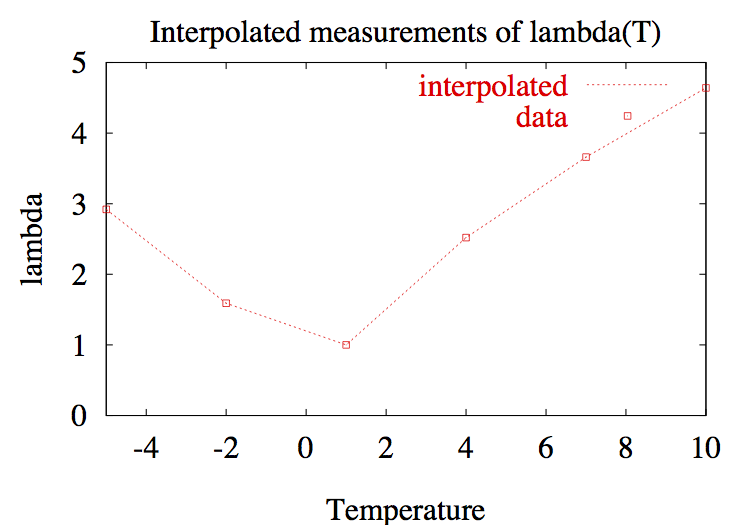
\includegraphics[height=3.5in]{table/table-interp.ps}}    \caption{A rock with $\lambda$\  known only at a sequence of
      discrete temperature values, from experimental measurements.
      The function $\lambda(T)$\   can be 
      represented approximately using linear interpolation (and the
      resulting approximate function can then be used to solve the
      problem numerically).}  \end{figure}
\end{example}%
\lthtmlfigureZ
\lthtmlcheckvsize\clearpage}

\stepcounter{subsection}
{\newpage\clearpage
\lthtmlfigureA{example251}%
\begin{example}
% latex2html id marker 251

  The rock in Example~\ref{lab1:exm:conduction} was considered to be small
  enough that the effects of heat diffusion in the interior
  were negligible in comparison to the heat lost by conduction
  through its surface.  
  In this example, consider a rock that is \emph{not small}, and whose
  temperature changes are dominated by internal diffusion effects.
  Therefore, it is no longer possible to ignore the spatial dependence
  in the problem.  
\par For simplicity, we will add spatial dependence in one direction
  only, which corresponds to a ``one-dimensional rock'', or a thin
  rod.  Assume that the rod is insulated along its sides, so that heat
  flows only along its length, and possibly out the ends (see
  Figure~\ref{lab1:fig:rock-1d}).
  \begin{figure}[htbp]
    \begin{center}
      \leavevmode
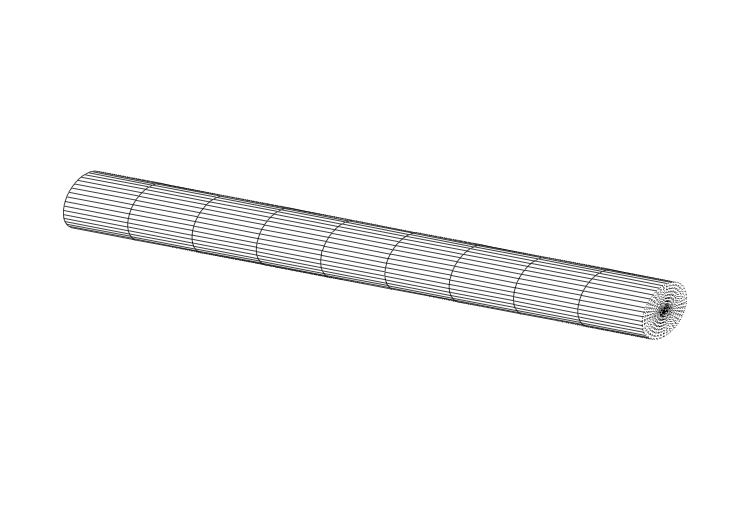
\includegraphics[width=4.5in,bb=50 100 410 250]{conduction/rod.eps}
      \caption{A thin rod can be thought of as a model for a
        one-dimensional rock.}    \end{center}
  \end{figure}
  Consequently, the temperature varies only with position, $x$, and
  time, $t$,
  and can be written as a function $u(x,t)$.   
  The temperature in the rod is governed by the following PDE
  \begin{displaymath}
    u_t = \alpha^2 u_{xx},
  \end{displaymath}
  for which we have to provide an initial temperature 
  \begin{displaymath} 
    u(x,0) = u_0(x),
  \end{displaymath}
  and boundary values
  \begin{displaymath}
    u(0,t)=u(1,t)=0,
  \end{displaymath}
  where 
  \begin{itemize}
  \item[$\circ$] $\alpha^2$\  is the \emph{thermal diffusivity} of the
    material, 
  \item[$\circ$] $u_0(x)$\  is the initial temperature distribution in the
    rod,  and
  \item[$\circ$] the boundary conditions indicate that the ends of the rod
    are held at constant temperature, which we've assumed is zero.
  \end{itemize}
\par Thermal diffusivity is a quantity that depends only on the
  material from which the bar is made.  It is defined by 
  \begin{displaymath}
  \alpha^2 = \frac{\kappa}{\rho c},
  \end{displaymath}
  where $\kappa$\  is the thermal conductivity, $\rho$\  is the density,
  and $c$\  is the specific heat.  A typical value of the thermal
  diffusivity for a granite 
  bar is $0.011\;cm^2/sec$, and $0.0038\;cm^2/sec$\  for a bar made of
  brick.  
\par Using the method of \emph{separation of variables}, we can look for a
  temperature function of the form $u(x,t)=X(x) \cdot T(t)$, which leads to
  the infinite series solution
  \begin{displaymath}
    u(x,t) = \sum_{n=1}^\infty b_n e^{-n^2\pi^2\alpha^2 t}\sin{(n\pi x)},
  \end{displaymath}
  where the series coefficients are
  \begin{displaymath}
    b_n = 2 \int_0^1 u_0(x) \sin{(n\pi x)} dx.
  \end{displaymath}
\par\begin{mathnote}
    Details of the derivation can be found in any introductory text in
    PDE's (for example, \cite[p.~549]{boyce-diprima}).  
  \end{mathnote}
\par We do manage to obtain an explicit formula for the solution, which can
  be used to calculate actual values of the solution.  However, there
  are two obvious reasons why this formula is not of much
  practical use:
  \begin{enumerate}
  \item The series involves an infinite number of terms (except for
    very special forms for the initial heat distribution \dots\ such as
    the one shown below).  
    We might be able to truncate the series, since each term
    decreases exponentially in size, but it is not trivial to decide
    how many terms to choose in order to get an accurate answer and 
    here we are already entering the realm of numerical
    approximation.  
  \item Each term in the series requires the evaluation of an
    integral.  When these cannot be integrated analytically, we must
    find some way to approximate the integrals \dots\ numerical
    analysis rears its head once again!
  \end{enumerate}
  For most physical problems, an analytical expression cannot be
  obtained, and the exact formula is not of much use.  
\par However, consider a very special case, when 
the initial temperature distribution is sinusoidal, i.e.~
  \begin{displaymath}
    u_0(x) = sin(\pi x).
  \end{displaymath}
  For this problem, the infinite series collapses into a single term
  \begin{displaymath}
    u(x,t) = e^{-\pi^2\alpha^2t}\sin{\pi x}.
  \end{displaymath}
\par\movie{exact.mpg}{Here is a movie of the exact solution to the
  diffusion problem.}
\par Notes on viewing movies:  Once the window comes-up on your screen
move the cursor into the movie window, otherwise the colour palette
is incorrect.  If no movie window comes-up it is probably because
there is no mpeg viewer on your system.
\par\end{example}%
\lthtmlfigureZ
\lthtmlcheckvsize\clearpage}

\stepcounter{paragraph}
\stepcounter{section}
{\newpage\clearpage
\lthtmlfigureA{example525}%
\begin{example}
% latex2html id marker 525

  We already saw an example of a discrete function in
  Example~\ref{lab1:exm:conduction-nonlinear}, where the rate function
  $\lambda$, depended on the temperature.
  If $\lambda$\  is not known by
  some empirical formula, then it can only be determined by
  experimental  
  measurements at a discrete set of temperature values. 
  In Figure~\ref{lab1:fig:table}, $\lambda$\  is given at a sequence of six
  temperature 
  points ( $(T_i, \lambda_i)$, for $i = 0, 1, \dots, 5)$\  ), and so is
  an example of a \emph{discrete function}.
\par The process of interpolation, which was introduced in
  Example~\ref{lab1:exm:conduction-nonlinear}, will be considered in more
  detail next.
\end{example}%
\lthtmlfigureZ
\lthtmlcheckvsize\clearpage}

{\newpage\clearpage
\lthtmlfigureA{example531}%
\begin{example}
% latex2html id marker 531

  Consider the two continuous functions 
  \begin{displaymath}
    f(x)=x^3-5x \;\; {\rm and} \;\; g(x)=x^{2/3} . 
  \end{displaymath}
  (In fact, $g(x)$\  was the function used to generate the values
  $\lambda(T)$\  in Example~\ref{lab1:exm:conduction-nonlinear}.)
\par The representation of functions using mathematical notation or
  graphs is very convenient for mathematicians, where continuous
  functions make sense.  However, a computer has a limited storage
  capacity, and so it can represent a function only at a finite number
  of discrete points $(x,y)$.
\par One question that arises immediately is: \emph{What do we do if we
    have to determine a value of the function which is not at one of
    the discrete points?}  
  The answer to this question is to use some form of {\em     interpolation} -- namely 
  to use an approximation procedure to estimate values of the function
  at points between the known values.
\par For example, linear interpolation approximates the function at
  intermediate points using the straight line segment joining the two
  neighbouring discrete points.
  There are other types of interpolation schemes that are more
  complicated, a few of which are:
  \begin{itemize}
  \item quadratic interpolation: every two sucessive points are joined
    by a quadratic polynomial.
  \item cubic splines: each pair of points is joined by a cubic
    polynomial so that the function values and first derivatives match
    at each point.
  \item Fourier series: instead of polynomials, uses a sum of 
    $\sin nx$\  and $\cos nx$\  to approximate the function (Fourier
    series are useful in analysis, as well as spectral methods).
  \item Chebyshev polynomials: another type of polynomial
    approximation which is useful for spectral methods.
  \item \dots many others \dots 
  \end{itemize}
  For details on any of these interpolation schemes, see a numerical
  analysis text such as that by \cite{burden-faires}.   
\par An application of linear interpolation to  discrete versions of
  the functions $f$\  and $g$\  is shown in
  Figure~\ref{lab1:fig:discrete-f}.
  \begin{figure}[htbp]
    \begin{center}
      \leavevmode
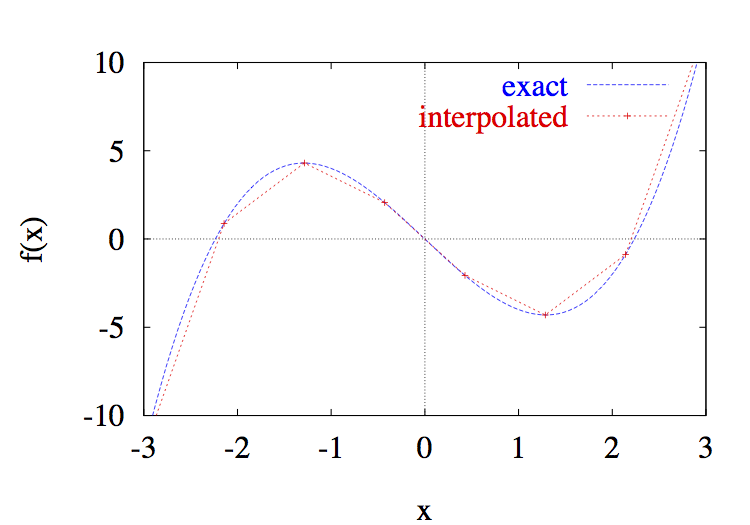
\includegraphics[height=3.5in]{discrete/f.eps}
      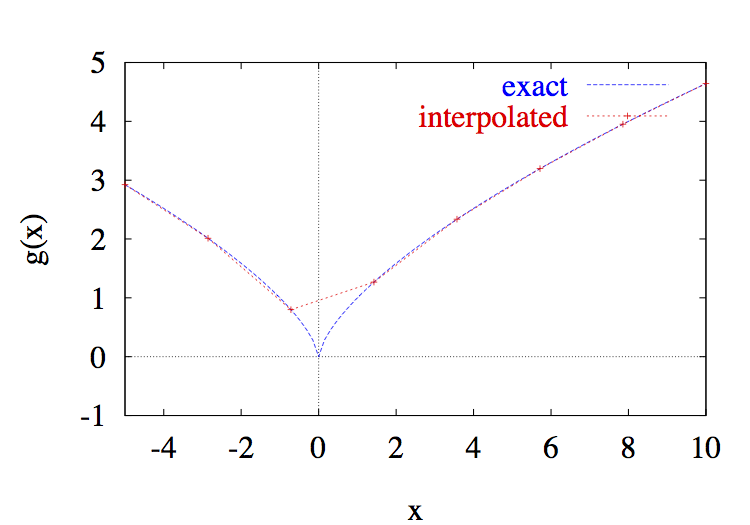
\includegraphics[height=3.5in]{discrete/g.eps}
      \caption{The functions $f$\  and $g$\  are known only at discrete
        points.  The function can be approximated at other values by
        linear interpolation, where straight line segments are used
        to join successive points.}    \end{center}
  \end{figure}
\par Depending on the function, or number of location of the points
  chosen, the approximation may be more or less accurate.  In
  Figure~\ref{lab1:fig:discrete-f}, it is not clear which function is
  approximated more accurately.  In the graph of $f(x)$, the error
  seems to be fairly small throughout.  However, for the function
  $g(x)$, the error is large near $x=0$, and then very small
  elsewhere.  
  This problem of \emph{accuracy} of
  discrete approximations will come up again and again in this course.
\par\demo{discrete.cgi}{Here is an interactive example demonstrating the
    use of interpolation (linear and cubic) in approximating
    functions.
}   
\par\technicalnote{Details on how the interpolation example works
  \dots}{See Appendix }{ for details on how the interpolation example
  works.}{lab1:tech:discrete}  
\par\quiz{quiz-interp.html}{After you finish the interpolation exercise, try
    out this short quiz.}
\end{example}%
\lthtmlfigureZ
\lthtmlcheckvsize\clearpage}

{\newpage\clearpage
\lthtmldisplayA{displaymath562}%
\begin{displaymath}
  \frac{dT}{dt} = -\lambda(T,t) \, (T-T_a),
\end{displaymath}%
\lthtmldisplayZ
\lthtmlcheckvsize\clearpage}

{\newpage\clearpage
\lthtmlinlinemathA{tex2html_wrap_inline668}%
$T(0)$%
\lthtmlinlinemathZ
\lthtmlcheckvsize\clearpage}

{\newpage\clearpage
\lthtmldisplayA{displaymath625}%
\begin{displaymath}
T_0, \, T_1, \, \ldots, \, T_i, \, \ldots,
\end{displaymath}%
\lthtmldisplayZ
\lthtmlcheckvsize\clearpage}

{\newpage\clearpage
\lthtmldisplayA{displaymath626}%
\begin{displaymath}
t_0<t_1<\cdots<t_i<\cdots.
\end{displaymath}%
\lthtmldisplayZ
\lthtmlcheckvsize\clearpage}

{\newpage\clearpage
\lthtmlinlinemathA{tex2html_wrap_inline672}%
$T_i$%
\lthtmlinlinemathZ
\lthtmlcheckvsize\clearpage}

{\newpage\clearpage
\lthtmlinlinemathA{tex2html_wrap_inline674}%
$t_i$%
\lthtmlinlinemathZ
\lthtmlcheckvsize\clearpage}

{\newpage\clearpage
\lthtmldisplayA{displaymath627}%
\begin{displaymath}
T_i \approx T(t_i).
\end{displaymath}%
\lthtmldisplayZ
\lthtmlcheckvsize\clearpage}

{\newpage\clearpage
\lthtmldisplayA{displaymath628}%
\begin{displaymath}
t_i=t_0+i \mbox{$\Delta t$}{}.
\end{displaymath}%
\lthtmldisplayZ
\lthtmlcheckvsize\clearpage}

{\newpage\clearpage
\lthtmlinlinemathA{tex2html_wrap_inline698}%
$t_i=t_0+i\mbox{$\Delta t$}{}$%
\lthtmlinlinemathZ
\lthtmlcheckvsize\clearpage}

{\newpage\clearpage
\lthtmlinlinemathA{tex2html_wrap_inline700}%
$i=0,1,2,\ldots$%
\lthtmlinlinemathZ
\lthtmlcheckvsize\clearpage}

{\newpage\clearpage
\lthtmlfigureA{figure568}%
\begin{figure}  \begin{center}
    \setlength{\unitlength}{4pt}    \leavevmode
    {\large     \begin{picture}(100,20)(0,10)
        \put(0,20){ \vector(1,0){90} }
        \put(93,19){$t$}
        \put(15,14){$t_0$}
        \put(15,20){ \circle*{1} }
        \put(25,14){$t_1$}
        \put(25,20){ \circle*{1} }
        \put(35,14){$t_2$}
        \put(35,20){ \circle*{1} }
        \put(45,20){ \circle*{1} }
        \put(49,14){$\cdots$}
        \put(55,20){ \circle*{1} }
        \put(65,14){$t_i$}
        \put(65,20){ \circle*{1} }
        \put(75,20){ \circle*{1} }
        \put(79,14){$\cdots$}
        \put(16,22.5){\vector(1,0){10}}
        \put(26,22.5){\vector(-1,0){10}}
        \put(19,24){\mbox{$\Delta t$}{}}
\end{picture}
    }
    \end{center}
\end{figure}%
\lthtmlfigureZ
\lthtmlcheckvsize\clearpage}

\stepcounter{paragraph}
\stepcounter{section}
{\newpage\clearpage
\lthtmlinlinemathA{tex2html_wrap_inline914}%
$y^\prime(t)$%
\lthtmlinlinemathZ
\lthtmlcheckvsize\clearpage}

{\newpage\clearpage
\lthtmldisplayA{displaymath764}%
\begin{displaymath}
  y^\prime(t) = \lim_{\mbox{$\Delta t$}{}\rightarrow 0} \frac{y(t+\mbox{$\Delta t$}{})-y(t)}{\mbox{$\Delta t$}{}}.
\end{displaymath}%
\lthtmldisplayZ
\lthtmlcheckvsize\clearpage}

{\newpage\clearpage
\lthtmlinlinemathA{tex2html_wrap_inline922}%
$dT/dt=T^\prime$%
\lthtmlinlinemathZ
\lthtmlcheckvsize\clearpage}

{\newpage\clearpage
\lthtmldisplayA{displaymath773}%
\begin{displaymath}
  T^\prime(t_i) \approx \frac{T_{i+1}-T_i}{\mbox{$\Delta t$}{}}.
\end{displaymath}%
\lthtmldisplayZ
\lthtmlcheckvsize\clearpage}

{\newpage\clearpage
\lthtmlfigureA{example778}%
\begin{example}
\demo{deriv.cgi}{Investigate the use of the forward difference
  formula to approximate derivatives here.
}
\par\technicalnote{Details on how the derivative example works
 \dots}{See Appendix }{ for details on how the derivative example
  works.}{lab1:tech:deriv} 
\par\end{example}%
\lthtmlfigureZ
\lthtmlcheckvsize\clearpage}

\stepcounter{subsection}
{\newpage\clearpage
\lthtmldisplayA{displaymath906}%
\begin{displaymath}
  \frac{T_{i+1}-T_i}{\mbox{$\Delta t$}{}} = \lambda(T_i,t_i) \, (T_i-T_a),
\end{displaymath}%
\lthtmldisplayZ
\lthtmlcheckvsize\clearpage}

{\newpage\clearpage
\lthtmldisplayA{displaymath794}%
\begin{displaymath}
  T_{i+1} = T_i + \mbox{$\Delta t$}{}\, \lambda(T_i,t_i) \, (T_i-T_a).
\end{displaymath}%
\lthtmldisplayZ
\lthtmlcheckvsize\clearpage}

{\newpage\clearpage
\lthtmlinlinemathA{tex2html_wrap_inline942}%
$y_{i+1} = y_i + \mbox{$\Delta t$}{}f(y_i,t_i)$%
\lthtmlinlinemathZ
\lthtmlcheckvsize\clearpage}

{\newpage\clearpage
\lthtmlfigureA{example803}%
\begin{example}
% latex2html id marker 803

  Let us now turn to another example in atmospheric physics to
  illustrate the use of the forward Euler method. 
  Consider the process of condensation and evaporation in a cloud. 
  The \emph{saturation ratio}, $S$, is the ratio of the vapour pressure
  to the vapour pressure of a plane surface of water at temperature
  $T$.  $S$\  varies in time according to the saturation development
  equation 
  \begin{equation}
    \frac{dS}{dt} = \alpha S^2 + \beta S + \gamma,
  \end{equation}
  where $\alpha$, $\beta$\  and $\gamma$\  are complicated (but constant)
  expressions involving the physical parameters in the problem (and so
  we won't reproduce them here).  
\par\begin{note}
    What are some physically reasonable values of the
    parameters (other than simply $\alpha<0$\  and $\gamma>0$)?   
  \end{note}
\par ~\cite{chen} gives a detailed derivation of the equation, which
  is a non-linear, first order ODE (i.e.~~non-linear in the dependent
  variable $S$, and it contains only a
  first derivative in the time variable). 
  Chen also derives an analytical solution to the problem which takes
  a couple pages of messy algebra to come to.
  Rather than show these
  details, we would like to use the forward Euler method in order to
  compute the solution numerically, and as we will see, this is
  actually quite simple.
\par Using the forward difference formula \eqref{lab1:eq:forward-diff}, the
  discrete form of~\eqref{lab1:eq:saturation} is 
  \begin{displaymath}
  S_{i+1} = S_i + \Delta t \left( \alpha S_i^2 + \beta S_i +
    \gamma \right).
  \end{displaymath}
  Consider an initial saturation ratio of $0.98$, and take parameter
  values $\alpha=-1$, $\beta=1$\  and $\gamma=1$.  
The resulting solution, for various values of the time step \mbox{$\Delta t$}{},is
  plotted in Figure~\ref{lab1:fig:saturation}. 
  \begin{figure}[htbp]
    \begin{center}
      \leavevmode
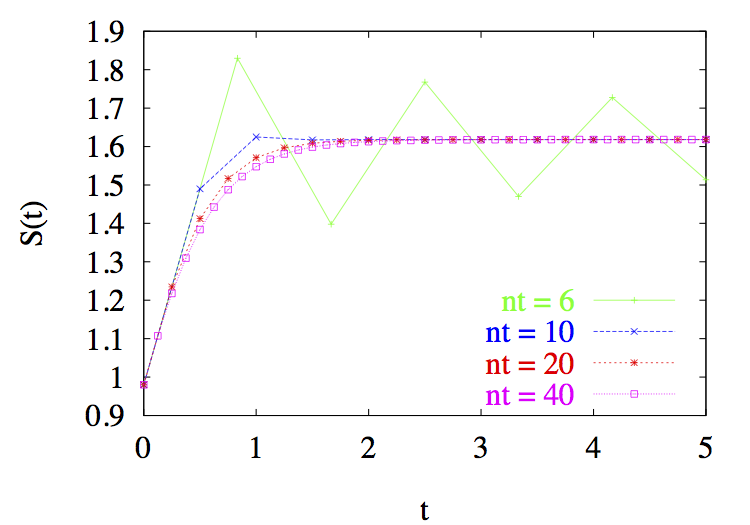
\includegraphics[height=3.5in]{feuler/sat2.eps}      
      \caption{Plot of the saturation ratio as a function of time
        using the Forward Euler method. ``{\tt{nt}}'' is the number of
        time steps.}    \end{center}
  \end{figure}
\par There are two things to notice here, both related to the importance of
  the choice of time step \mbox{$\Delta t$}{}\ :
  \begin{itemize}
  \item As \mbox{$\Delta t$}{}\ is reduced, the solution appears to \emph{converge}
    to one solution curve, which we would hope is the exact solution
    to the differential equation.  An important question to ask is:
    \emph{When will the numerical method converge to the exact
      solution as \mbox{$\Delta t$}{}\ is reduced?}   
  \item If \mbox{$\Delta t$}{}\ is taken too large, however, the numerical solution
    breaks down.  In the above example, the oscillations that occur
    for the largest time step (when $nt=6$) are a sign of {\em       numerical instability}.  The differential problem is stable
    and exhibits no such behaviour, but the numerical scheme we have
    used has introduced an instability.
    An obvious question that arises is: \emph{How can we avoid
      introducing instabilities in a numerical scheme?}
  \end{itemize}
  Neither question has an obvious answer, and both issues will be
  investigated further in \htmladdnormallink{Lab~\#2}{\LabtwoURL}
\end{example}%
\lthtmlfigureZ
\lthtmlcheckvsize\clearpage}

\stepcounter{subsection}
{\newpage\clearpage
\lthtmlinlinemathA{tex2html_wrap_inline982}%
$T^\prime$%
\lthtmlinlinemathZ
\lthtmlcheckvsize\clearpage}

{\newpage\clearpage
\lthtmldisplayA{displaymath836}%
\begin{displaymath}
  T^\prime(t) = \lim_{\mbox{$\Delta t$}{}\rightarrow 0} \frac{T(t)-T(t-\mbox{$\Delta t$}{})}{\mbox{$\Delta t$}{}}.
\end{displaymath}%
\lthtmldisplayZ
\lthtmlcheckvsize\clearpage}

{\newpage\clearpage
\lthtmldisplayA{displaymath843}%
\begin{displaymath}
  T^\prime(t_i) \approx \frac{T_i-T_{i-1}}{\mbox{$\Delta t$}{}},
\end{displaymath}%
\lthtmldisplayZ
\lthtmlcheckvsize\clearpage}

{\newpage\clearpage
\lthtmldisplayA{displaymath849}%
\begin{displaymath}
  T^\prime(t_i) \approx \frac{T_{i+1}-T_{i-1}}{2 \mbox{$\Delta t$}{}}.
\end{displaymath}%
\lthtmldisplayZ
\lthtmlcheckvsize\clearpage}

\stepcounter{paragraph}
\stepcounter{section}
\stepcounter{subsection}
{\newpage\clearpage
\lthtmldisplayA{displaymath1047}%
\begin{displaymath}
  y^{\prime\prime}(t_i) \approx 
  \frac{y(t_{i+1})-2y(t_i)+y(t_{i-1})}{(\mbox{$\Delta t$}{})^2} ,
\end{displaymath}%
\lthtmldisplayZ
\lthtmlcheckvsize\clearpage}

{\newpage\clearpage
\lthtmlfigureA{example1056}%
\begin{example}
% latex2html id marker 1056

  A weather balloon, filled with helium, climbs vertically until it
  reaches its level of neutral buoyancy, at which point it begins to
  oscillate about this equilibrium height.  We can derive a DE
  describing the motion of the balloon by applying Newton's second
  law:  
  \begin{displaymath}
    mass \; \times \; acceleration = force 
  \end{displaymath}
  \begin{displaymath}
    m \frac{d^2 y}{d t^2} = 
      \underbrace{- \beta \frac{dy}{dt}}_{\mbox{\rm air resistance}} 
      \underbrace{- \gamma y}_{\mbox{\rm buoyant force}},
  \end{displaymath}
  where
  \begin{itemize}
  \item[\ ] $y(t)$\  is the displacement of the balloon vertically from
    its equilibrium level, $y=0$; 
  \item[\ ] $m$\  is the mass of the balloon and payload;
  \item[\ ] the oscillations are assumed small, so that we can
    assume a linear functional form for the buoyant force, 
    $-\gamma y$.
  \end{itemize}
  This problem also requires initial values for both the initial
  displacement and velocity:
  \begin{displaymath} 
    y(0) = y_0 \;\; \mbox{\rm and} \;\; \frac{dy}{dt}(0) = v_0.
  \end{displaymath}
\par\begin{figure}[htbp]
    \begin{center}
      \leavevmode
      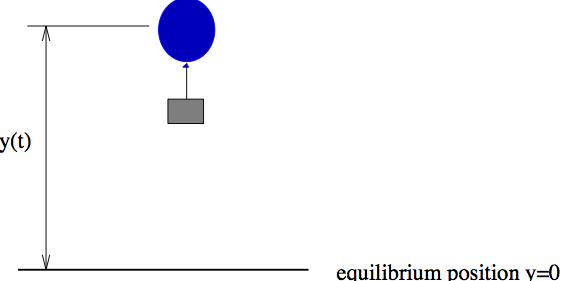
\includegraphics{balloon/balloon.eps}
      \caption{A weather balloon oscillating about its level of
        neutral buoyancy.}    \end{center}
  \end{figure}
\end{example}%
\lthtmlfigureZ
\lthtmlcheckvsize\clearpage}

{\newpage\clearpage
\lthtmlfigureA{problem1078}%
\begin{problem}
% latex2html id marker 1078

  \begin {itemize}
  \item a)
  Using the centered difference formula~\eqref{lab1:eq:centered-diff2}
  for the second derivative, and the forward difference
  formula~\eqref{lab1:eq:forward-diff} for the first derivative at the
  point $t_i$, derive a difference scheme for $y_{i+1}$, the vertical
  displacement of the weather balloon.
\par\item b)
  What is the difference between this scheme and the forward
  Euler scheme from Example~\ref{lab1:exm:saturation}, related to the
  initial conditions?  (\textbf{Hint:} think about starting values \dots)
\par\item c)
   Given the initial values above, explain how to start the numerical
  integration.
\par\end {itemize}
\end{problem}%
\lthtmlfigureZ
\lthtmlcheckvsize\clearpage}

\stepcounter{subsection}
{\newpage\clearpage
\lthtmlfigureA{example1090}%
\begin{example}
% latex2html id marker 1090

  The second order DE for the weather balloon problem from
  Example~\ref{lab1:exm:balloon}
  can be rewritten by letting $u=dy/dt$.  Then,
  \begin{displaymath}
    \frac{dy}{dt} = u 
  \end{displaymath}
  \begin{displaymath}
    \frac{du}{dt} = -\frac{\beta}{m} u - \frac{\gamma}{m} y
  \end{displaymath}
  which is a system of first order ODE's in $u$\  and $y$.  
  This set of differential equations can be discretized to obtain
  another numerical scheme for the weather balloon problem.
\end{example}%
\lthtmlfigureZ
\lthtmlcheckvsize\clearpage}

{\newpage\clearpage
\lthtmlfigureA{problem1101}%
\begin{problem}
  \begin{itemize}
  \item a)
  Derive a difference scheme for the problem based on the
  above system of two ODE's using the forward difference formula for
  the first derivative. 
\par\item  b)
  By combining the discretized equations into  one  equation for y,
 show that the difference between this scheme and the scheme  obtained
 in problem one is the difference formula for the second derivative.
\par\end {itemize}
\par\end{problem}%
\lthtmlfigureZ
\lthtmlcheckvsize\clearpage}

\stepcounter{subsection}
{\newpage\clearpage
\lthtmlinlinemathA{tex2html_wrap_inline1218}%
$\partial u/\partial t = 0$%
\lthtmlinlinemathZ
\lthtmlcheckvsize\clearpage}

{\newpage\clearpage
\lthtmlinlinemathA{tex2html_wrap_inline1220}%
$u_(x)$%
\lthtmlinlinemathZ
\lthtmlcheckvsize\clearpage}

{\newpage\clearpage
\lthtmldisplayA{displaymath1171}%
\begin{displaymath} u_{xx} = 0, \end{displaymath}%
\lthtmldisplayZ
\lthtmlcheckvsize\clearpage}

{\newpage\clearpage
\lthtmldisplayA{displaymath1172}%
\begin{displaymath} u(0) = u(1) = 0. \end{displaymath}%
\lthtmldisplayZ
\lthtmlcheckvsize\clearpage}

{\newpage\clearpage
\lthtmlfigureA{example1121}%
\begin{example}
  We can discretize the steady state diffusion equation using the
  centered difference formula~\eqref{lab1:eq:centered-diff2} for the
  second derivative to obtain:
  \begin{displaymath}
  u_{i+1}-2u_i+u_{i-1} = 0
  \end{displaymath}
  where $u_i\approx u(i/N)$\  and $i=0,1,\ldots,N$\  (and the factor of
  $(\Delta x)^2 = {1}/{N^2}$\  has been multiplied out).  
  The boundary values $u_0$\  and $u_N$\  are both known to be zero, so
  the above expression represents a system of $N-1$\  equations in $N-1$  unknown values $u_i$\  that must be solved for \emph{simultaneously}.
  The solution of such systems of linear equations will be covered in
  more detail in \htmladdnormallink{Lab~\#3}{\LabthreeURL} $-$\  in
  fact, this equation forms the basis for a Problem in the
  Linear Algebra Lab~\externalref{lab3:sec:prob}.
\par Compare this to the initial value problems discretized using the
  forward Euler method, where the resulting numerical scheme is
  a step-by-step, marching process (that is, the solution at one grid
  point can be computed using an explicit formula using only the value
  at the previous grid point).
\end{example}%
\lthtmlfigureZ
\lthtmlcheckvsize\clearpage}

\stepcounter{subsection}
{\newpage\clearpage
\lthtmlfigureA{example1134}%
\begin{example}
% latex2html id marker 1134

  To illustrate the process, let us go back to the heat diffusion
  problem from Example~\ref{lab1:exm:diffusion1d}, an initial-boundary
  value problem in the temperature $u(x,t)$:
  \begin{displaymath}
  u_{t} = \alpha^2 u_{xx},
  \end{displaymath}
  along with initial values
  \begin{displaymath}
  u(x,0) = u_0(x),
  \end{displaymath}
  and boundary values
  \begin{displaymath}
  u(0,t) = u(1,t) = 0.
  \end{displaymath}
\par As for ODE's, the steps in the process of discretization remain the
  same:
  \begin{enumerate}
  \item First, replace the independent variables by discrete values
    \begin{displaymath}
    x_i = i \Delta x = \frac{i}{M}, \;\; \mbox{\rm where $i=0, 1,
      \ldots, M$, and}
    \end{displaymath}
    \begin{displaymath}
    t_n = n \Delta t, \;\; \mbox{\rm where $n=0, 1,
      \ldots$}
    \end{displaymath}
    In this example, the set of discrete points define a two-dimensional
    grid of points, as pictured in Figure~\ref{lab1:fig:pde-grid}.
    \begin{figure}[htbp]
      \begin{center}
        \leavevmode
        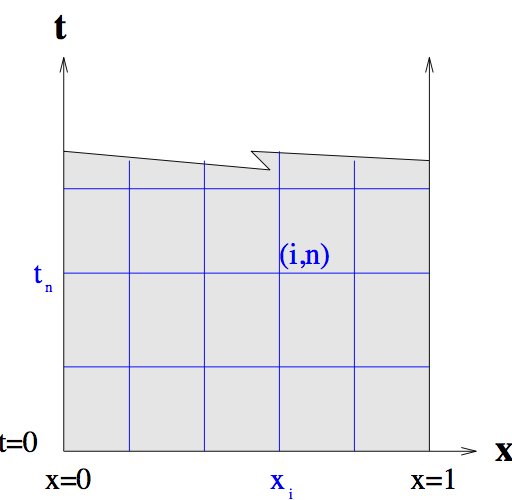
\includegraphics{pdes/pde-grid.eps}
        \caption{The computational grid for the heat diffusion problem,
          with discrete points $(x_i,t_n)$.}      \end{center}
    \end{figure}
\par\item Replace the dependent variables (in this example, just the
    temperature $u(x,t)$) with approximations defined at the grid
    points:
    \begin{displaymath} 
    U_i^n \approx u(x_i,t_n).
    \end{displaymath}
    The boundary and initial values for the discrete temperatures can then
    be written in terms of the given information.
\par\item Approximate all of the derivatives appearing in the problem with
    finite difference approximations.  
    If we use the centered difference
    approximation~\eqref{lab1:eq:centered-diff2} for the second
    derivative in $x$, and the forward difference
    formula~\eqref{lab1:eq:forward-diff} for the time derivative
    (while evaluating the terms on the right hand side at the previous
    time level), we obtain the following numerical scheme:
    \begin{displaymath}
    U_i^{n+1} = U_i^n + \frac{\alpha^2 \Delta t}{(\Delta x)^2} \left(
      U_{i+1}^n - 2 U_i^n + U_{i-1}^n \right).
    \end{displaymath}
  \end{enumerate}
  Given the initial values, $U_i^0=u_0(x_i)$,
  and boundary values $U_0^n=U_M^n=0$, this difference formula allows
  us to compute values of temperature at any time, based on
  values at the previous time.
\par There are, of course, other ways of discretizing this problem, but
  the above is one of the simplest.  
\end{example}%
\lthtmlfigureZ
\lthtmlcheckvsize\clearpage}

\appendix
\stepcounter{section}
\stepcounter{subsection}
{\newpage\clearpage
\lthtmldisplayA{displaymath1350}%
\begin{displaymath}
  \frac{dT}{dt} = -\lambda (T-T_a),
\end{displaymath}%
\lthtmldisplayZ
\lthtmlcheckvsize\clearpage}

{\newpage\clearpage
\lthtmlinlinemathA{tex2html_wrap_inline1364}%
$T$%
\lthtmlinlinemathZ
\lthtmlcheckvsize\clearpage}

{\newpage\clearpage
\lthtmldisplayA{displaymath1351}%
\begin{displaymath}
  \frac{dT}{T-T_a} = -\lambda dt.
\end{displaymath}%
\lthtmldisplayZ
\lthtmlcheckvsize\clearpage}

{\newpage\clearpage
\lthtmlinlinemathA{tex2html_wrap_inline1366}%
$0$%
\lthtmlinlinemathZ
\lthtmlcheckvsize\clearpage}

{\newpage\clearpage
\lthtmldisplayA{displaymath1352}%
\begin{displaymath}
  \int_{T(0)}^{T(t)} \frac{dS}{S-T_a} = -\int_0^t\lambda ds,
\end{displaymath}%
\lthtmldisplayZ
\lthtmlcheckvsize\clearpage}

{\newpage\clearpage
\lthtmlinlinemathA{tex2html_wrap_inline1370}%
$s$%
\lthtmlinlinemathZ
\lthtmlcheckvsize\clearpage}

{\newpage\clearpage
\lthtmlinlinemathA{tex2html_wrap_inline1372}%
$S$%
\lthtmlinlinemathZ
\lthtmlcheckvsize\clearpage}

{\newpage\clearpage
\lthtmldisplayA{displaymath1353}%
\begin{displaymath}
  \ln \left( T(t)-T_a)-\ln(T(0)-T_a \right) = -\lambda t,
\end{displaymath}%
\lthtmldisplayZ
\lthtmlcheckvsize\clearpage}

{\newpage\clearpage
\lthtmldisplayA{displaymath1354}%
\begin{displaymath}
  T(t) = T_a + (T(0)-T_a)e^{-\lambda t},
\end{displaymath}%
\lthtmldisplayZ
\lthtmlcheckvsize\clearpage}

\stepcounter{section}
\stepcounter{subsection}
\stepcounter{subsection}
{\newpage\clearpage
\lthtmlinlinemathA{tex2html_wrap_inline1431}%
$f(x)$%
\lthtmlinlinemathZ
\lthtmlcheckvsize\clearpage}

{\newpage\clearpage
\lthtmlinlinemathA{tex2html_wrap_inline1433}%
$g(x)$%
\lthtmlinlinemathZ
\lthtmlcheckvsize\clearpage}

\stepcounter{subsection}

\end{document}
